\documentclass[11pt,a4paper]{article}

% -----------------------------------------------------------------------------
% Page setup
% -----------------------------------------------------------------------------
\usepackage[a4paper,margin=1in]{geometry}
\usepackage[T1]{fontenc}
\usepackage[utf8]{inputenc}
\usepackage{lmodern}
\usepackage{amsmath,amssymb,bm,mathtools}
\usepackage{booktabs,longtable,array,tabularx}
\usepackage{enumitem}
\usepackage{xcolor}
\usepackage{hyperref}
\usepackage{xurl}
\usepackage{listings}
\usepackage{caption}
\usepackage{float}
\usepackage{tikz}
\usetikzlibrary{positioning}
\usepackage{fancyhdr}
\usepackage{microtype}

\hypersetup{
  colorlinks=true,
  linkcolor=blue!55!black,
  urlcolor=blue!55!black,
  citecolor=blue!55!black,
  pdftitle={Network Optimal Control and Differential Games: Code Walkthrough and Model Adaptation Guide},
  pdfauthor={Lu-Xing Yang}
}

\setlength{\headheight}{14pt}
\pagestyle{fancy}
\fancyhf{}
\lhead{Network Control and Differential Games}
\rhead{Code Walkthrough}
\cfoot{\thepage}

\setlist[itemize]{topsep=3pt,itemsep=2pt,parsep=0pt,leftmargin=1.8em}
\setlist[enumerate]{topsep=3pt,itemsep=2pt,parsep=0pt,leftmargin=1.9em}
\renewcommand{\arraystretch}{1.22}

\definecolor{codebg}{RGB}{248,248,248}
\definecolor{codeframe}{RGB}{220,220,220}
\definecolor{keywordblue}{RGB}{20,80,150}
\definecolor{commentgreen}{RGB}{35,120,60}
\definecolor{stringred}{RGB}{150,40,40}

\lstdefinestyle{py}{
  language=Python,
  basicstyle=\ttfamily\small,
  backgroundcolor=\color{codebg},
  frame=single,
  rulecolor=\color{codeframe},
  breaklines=true,
  columns=fullflexible,
  showstringspaces=false,
  keywordstyle=\color{keywordblue}\bfseries,
  commentstyle=\color{commentgreen},
  stringstyle=\color{stringred},
  tabsize=4
}
\lstdefinestyle{bash}{
  language=bash,
  basicstyle=\ttfamily\small,
  backgroundcolor=\color{codebg},
  frame=single,
  rulecolor=\color{codeframe},
  breaklines=true,
  columns=fullflexible,
  showstringspaces=false,
  tabsize=2
}
\lstdefinestyle{text}{
  basicstyle=\ttfamily\small,
  backgroundcolor=\color{codebg},
  frame=single,
  rulecolor=\color{codeframe},
  breaklines=true,
  columns=fullflexible,
  showstringspaces=false
}

\DeclareRobustCommand{\code}[1]{\texttt{\detokenize{#1}}}
\newcommand{\dd}{\,\mathrm{d}}
\newcommand{\R}{\mathbb{R}}
\newcommand{\Proj}{\operatorname{Proj}}

\title{\bfseries Network Optimal Control and Differential Games\\[2mm]
\large Code Walkthrough and Model Adaptation Guide}
\author{Lu-Xing Yang}
\date{\today}

\begin{document}
\maketitle

\begin{abstract}
This document explains how to run and modify two Python teaching scripts for network optimal control, differential games, and hybrid or impulsive interventions. It covers how to read realistic network data, compute an empirical degree distribution, convert a network into the adjacency matrix required by node-level models, implement degree-class and node-level dynamics, and modify the state equation, Jacobian, objective functional, Hamiltonian update rule, and impulse jump structure for other models. The numerical solvers are based on Pontryagin's maximum principle (PMP) and the forward-backward sweep method. In the game examples, the computed controls should be interpreted as open-loop Nash candidates satisfying necessary optimality conditions, not as automatically guaranteed global optima. For research use, they should be checked against no-control, constant-control, random-control, and unilateral-deviation baselines.
\end{abstract}

\paragraph{Author note.}
This guide was created from my research experience in optimal control, differential games, hybrid/impulsive control, and cyber/network-security applications over the past few years. The perspective is informed by publications in venues including IEEE TIFS, TDSC, TSMC, TNSE, TCSS, and related journals.

\tableofcontents
\newpage

% -----------------------------------------------------------------------------
\section{Purpose and Code Files}

The tutorial package uses a simple-to-extended structure. The two most important files are:

\begin{lstlisting}[style=text]
code/simple_degree_k_control.py
code/network_control_examples.py
\end{lstlisting}

\code{simple_degree_k_control.py} is the recommended starting point. It implements one complete degree-class optimal-control example. It loads a network, computes the empirical degree distribution, builds a degree-\(k\) SIS-type control model, solves the PMP system by a forward-backward sweep, and writes figures and CSV summaries.

\code{network_control_examples.py} is a compact extension script. It keeps the code in one readable file, but adds a degree-level attacker-defender differential game, node-level adjacency-matrix control and game models, a hybrid/impulsive simulation template, and additional input formats for realistic network data.

The intended reading order is:

\begin{center}
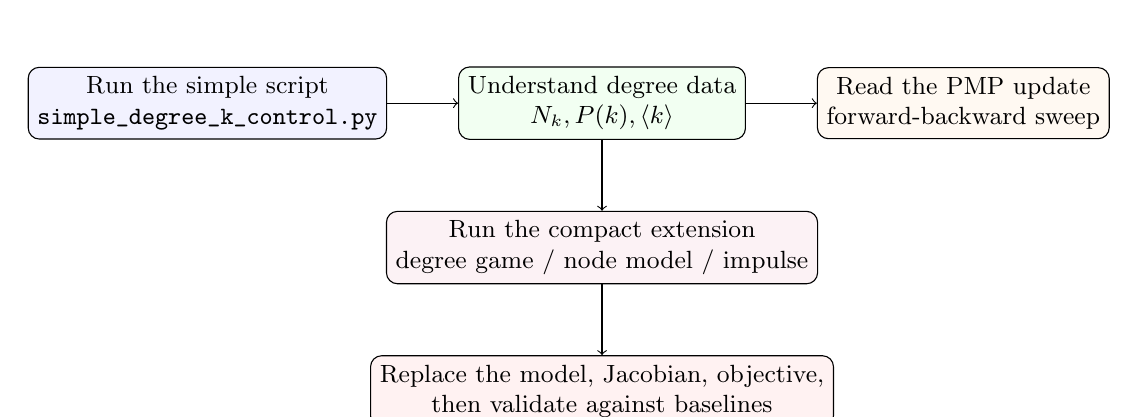
\begin{tikzpicture}[node distance=7mm, every node/.style={font=\small}]
\node[draw, rounded corners, fill=blue!5, align=center, minimum width=34mm] (a) {Run the simple script\\\code{simple_degree_k_control.py}};
\node[draw, rounded corners, fill=green!5, align=center, right=9mm of a, minimum width=34mm] (b) {Understand degree data\\\(N_k,P(k),\langle k\rangle\)};
\node[draw, rounded corners, fill=orange!5, align=center, right=9mm of b, minimum width=34mm] (c) {Read the PMP update\\forward-backward sweep};
\node[draw, rounded corners, fill=purple!5, align=center, below=9mm of b, minimum width=47mm] (d) {Run the compact extension\\degree game / node model / impulse};
\node[draw, rounded corners, fill=red!5, align=center, below=9mm of d, minimum width=50mm] (e) {Replace the model, Jacobian, objective,\\then validate against baselines};
\draw[->] (a) -- (b);
\draw[->] (b) -- (c);
\draw[->] (b) -- (d);
\draw[->] (d) -- (e);
\end{tikzpicture}
\end{center}

% -----------------------------------------------------------------------------
\section{Environment Setup and Basic Execution}

From the public repository root, a virtual environment is recommended:

\begin{lstlisting}[style=bash]
git clone https://github.com/LYang910920/network-control-differential-games.git
cd network-control-differential-games

python -m venv .venv
source .venv/bin/activate        # macOS / Linux
# .venv\Scripts\activate         # Windows PowerShell

python -m pip install -r requirements.txt
\end{lstlisting}

Run all lecture examples from the repository root:

\begin{lstlisting}[style=bash]
python run_all.py --skip-reference
\end{lstlisting}

For the direct script commands below, move into the lecture-example folder:

\begin{lstlisting}[style=bash]
cd examples/lecture
\end{lstlisting}

Then run the simple degree-\(k\) example first:

\begin{lstlisting}[style=bash]
python code/simple_degree_k_control.py
\end{lstlisting}

By default, it creates a Barabasi-Albert demo network, computes the empirical degree distribution, and solves a degree-class optimal-control problem. The output folder is:

\begin{lstlisting}[style=text]
simple_outputs/
  degree_distribution.csv
  degree_distribution.png
  degree_k_control.png
\end{lstlisting}

Then run the compact extension example:

\begin{lstlisting}[style=bash]
python code/network_control_examples.py
\end{lstlisting}

The default output folder is:

\begin{lstlisting}[style=text]
example_outputs/
  degree_distribution.csv
  degree_distribution.png
  degree_control.png
  degree_game.png
  node_control.png
  node_game.png
  hybrid_impulse.png
\end{lstlisting}

You may also run only selected model groups:

\begin{lstlisting}[style=bash]
python code/network_control_examples.py --examples degree
python code/network_control_examples.py --examples node
python code/network_control_examples.py --examples hybrid
\end{lstlisting}

% -----------------------------------------------------------------------------
\section{Using Realistic Network Data}

\subsection{Edge-list data}

The most common network format is an edge list. For example, suppose a CSV file is:

\begin{lstlisting}[style=text]
source,target,weight
1,2,1.0
2,3,2.0
3,5,1.0
\end{lstlisting}

Run:

\begin{lstlisting}[style=bash]
python code/network_control_examples.py \
  --edge-list sample_data/sample_edges.csv \
  --delimiter , \
  --has-header \
  --source-col source \
  --target-col target \
  --weight-col weight \
  --max-nodes 50
\end{lstlisting}

The argument \code{--max-nodes 50} only limits the dense node-level adjacency matrix used in the node-level examples. It does not truncate the network before computing the empirical degree distribution. This is intentional: the degree-level model should reflect the whole input network, while the node-level model may be restricted for a small teaching example.

If the edge-list file has no header and the first two columns are source and target, use column indices:

\begin{lstlisting}[style=bash]
python code/network_control_examples.py \
  --edge-list data/edges.txt \
  --delimiter ' ' \
  --source-col 0 \
  --target-col 1
\end{lstlisting}

\subsection{Adjacency-matrix CSV}

If the input is already an adjacency matrix CSV, run:

\begin{lstlisting}[style=bash]
python code/network_control_examples.py \
  --adjacency-csv sample_data/sample_adjacency.csv
\end{lstlisting}

The node-level ODE convention used in the script is:
\[
  \text{pressure}=A x,
  \qquad
  A[i,j]=\text{influence from node }j\text{ to node }i.
\]
That is, the \(i\)-th component of \(Ax\) is the total influence received by node \(i\). If your CSV is already in this model convention, use:

\begin{lstlisting}[style=bash]
python code/network_control_examples.py \
  --adjacency-csv sample_data/sample_adjacency.csv \
  --adjacency-convention model
\end{lstlisting}

If your CSV follows the usual graph convention where \(A[i,j]\) means an edge from node \(i\) to node \(j\), the script can transpose it internally for directed influence models.

\subsection{Directed networks and degree modes}

For directed networks, the degree distribution can be computed in several ways:

\begin{lstlisting}[style=text]
undirected   treat the network as undirected; useful for contact or infection spreading
in           use in-degree; useful for measuring how much influence a node receives
out          use out-degree; useful for measuring how much influence a node can exert
total        use in-degree plus out-degree
\end{lstlisting}

Example:

\begin{lstlisting}[style=bash]
python code/network_control_examples.py \
  --edge-list data/edges.csv \
  --delimiter , \
  --has-header \
  --directed \
  --degree-mode in
\end{lstlisting}

For degree-level mean-field models, choose the degree mode according to the model interpretation. In a rumor or malware-contact model, an undirected or total degree is often natural. In an information-influence model, in-degree and out-degree may play different roles.

% -----------------------------------------------------------------------------
\section{Core Mathematical Conventions}

\subsection{Degree-level arrays are indexed by degree class}

The degree-level implementation is not a compartment-level implementation. The columns of the state array are indexed by observed degree values. If the network has degree classes
\[
  k_1,k_2,\ldots,k_m,
\]
then the state and control arrays are organized as
\[
  X[:,j] = x_{k_j}(t),
  \qquad
  U[:,j] = u_{k_j}(t).
\]
For example,

\begin{lstlisting}[style=text]
degrees = [1, 2, 4, 7]
X[:, 0] = infected fraction among degree-1 nodes
X[:, 1] = infected fraction among degree-2 nodes
X[:, 2] = infected fraction among degree-4 nodes
X[:, 3] = infected fraction among degree-7 nodes
\end{lstlisting}

The code first computes
\[
  N_k = \#\{\text{nodes with degree }k\},
  \qquad
  P(k)=\frac{N_k}{n},
  \qquad
  \langle k\rangle = \sum_k kP(k).
\]
The mean-field infection pressure is
\[
  \Theta(t)=\frac{\sum_k kP(k)x_k(t)}{\langle k\rangle}.
\]
This quantity can be interpreted as the probability that a randomly selected edge points to an infected node under the degree-based mean-field approximation.

\subsection{Node-level arrays are indexed by nodes}

In the node-level implementation, the state vector is indexed by node:
\[
  x(t)=(x_1(t),\ldots,x_n(t))^\top.
\]
The influence term is computed by matrix multiplication:
\[
  A x,
\]
where \(A[i,j]\) is the influence from node \(j\) to node \(i\). A typical node-level SIS-control equation is
\[
  \dot{x}_i(t)
  =\beta(1-x_i(t))\sum_j A_{ij}x_j(t)
  -(\delta+u_i(t))x_i(t).
\]
Node-level models are more detailed but computationally more expensive, because the Jacobian is \(n\times n\) and must be evaluated repeatedly during the forward-backward sweep.

% -----------------------------------------------------------------------------
\section[Simple Script: simple\_degree\_k\_control.py]{Simple Script: \texttt{simple\_degree\_k\_control.py}}

\subsection{Main workflow}

The simple script follows one clean teaching pipeline:

\begin{lstlisting}[style=text]
load network
-> compute degree distribution
-> build degree-k SIS dynamics
-> solve the forward state equation
-> solve the backward adjoint equation
-> update the control from Hamiltonian stationarity
-> save figures and CSV files
\end{lstlisting}

The central function is conceptually:

\begin{lstlisting}[style=py]
solve_degree_k_control(...)
\end{lstlisting}

It returns the time grid, degree classes, state trajectory, control trajectory, adjoint trajectory, and objective value.

\subsection{Network loading}

The network-loading function supports three cases:

\begin{lstlisting}[style=text]
--edge-list       edge-list file
--adjacency-csv   adjacency matrix CSV
no input          built-in Barabasi-Albert demo graph
\end{lstlisting}

For edge lists, the script reads the table with \code{pandas.read_csv} and converts it to a NetworkX graph. For an adjacency CSV, it reads a square matrix and converts it to a graph. The simple script uses an undirected graph by default, because the example is a contact-spreading model.

\subsection{Degree distribution}

The core degree-distribution function returns
\[
  k,\quad N_k,\quad P(k),\quad \langle k\rangle.
\]
In code, the key outputs are:

\begin{lstlisting}[style=py]
k, counts, p, kbar = degree_distribution(G)
\end{lstlisting}

Here \code{k} is a one-dimensional array of observed degree classes, \code{counts} stores \(N_k\), \code{p} stores \(P(k)\), and \code{kbar} stores the average degree \(\langle k\rangle\).

The degree-level state and control arrays have shape:

\begin{lstlisting}[style=text]
X.shape = (number_of_time_points, number_of_degree_classes)
U.shape = (number_of_time_points, number_of_degree_classes)
\end{lstlisting}

\subsection{Degree-\(k\) SIS control model}

The simple model is
\[
  \dot{x}_k(t)
  =\beta k(1-x_k(t))\Theta(t)
  -(\delta+u_k(t))x_k(t),
\]
where
\[
  \Theta(t)=\frac{\sum_k kP(k)x_k(t)}{\langle k\rangle}.
\]
The control \(u_k(t)\) increases the removal, recovery, repair, or suppression rate for degree class \(k\). The code implements this equation as:

\begin{lstlisting}[style=py]
def theta(x, k, p, kbar):
    return float((k * p) @ x / max(kbar, 1e-12))

def state_rhs(x, u, k, p, kbar, beta, delta):
    return beta * k * (1.0 - x) * theta(x, k, p, kbar) - (delta + u) * x
\end{lstlisting}

A typical running cost is
\[
  L(x,u)=q\sum_k P(k)x_k+\frac{r}{2}\sum_kP(k)u_k^2.
\]
The first term penalizes prevalence. The second term penalizes control effort.

\subsection{PMP and the forward-backward sweep}

For a minimization problem with Hamiltonian
\[
  H(x,u,\lambda)=L(x,u)+\lambda^\top f(x,u),
\]
the adjoint equation is
\[
  \dot{\lambda}(t)
  =-\frac{\partial L}{\partial x}(x(t),u(t))
   -f_x(x(t),u(t))^\top\lambda(t),
  \qquad
  \lambda(T)=0,
\]
when there is no terminal cost. The forward-backward sweep repeats:

\begin{lstlisting}[style=text]
initialize U(t)
repeat:
    1. solve the state equation forward from x(0)
    2. solve the adjoint equation backward from lambda(T)
    3. update U(t) from Hamiltonian stationarity
until convergence or max iterations
\end{lstlisting}

In the simple SIS-control model,
\[
  \frac{\partial f_k}{\partial u_k}=-x_k.
\]
Stationarity gives
\[
  0=\frac{\partial H}{\partial u_k}
   = rP(k)u_k-\lambda_kx_k.
\]
Thus,
\[
  u_k^*(t)
  =\Proj_{[0,u_{\max}]}
  \left(
    \frac{\lambda_k(t)x_k(t)}{rP(k)}
  \right).
\]
The code implements the projection and a damping step:

\begin{lstlisting}[style=py]
candidate = Lambda * X / (control_weight * np.maximum(p, 1e-12))
U_new = np.clip(candidate, 0.0, u_max)
U = damping * U_new + (1.0 - damping) * U_old
\end{lstlisting}

The damping factor is important. Nonlinear PMP boundary-value iterations can oscillate or diverge if the control is updated too aggressively.

% -----------------------------------------------------------------------------
\section[Compact Extension: network\_control\_examples.py]{Compact Extension: \texttt{network\_control\_examples.py}}

\subsection{Overall structure}

The extension script remains a single file, but its internal sections are organized as:

\begin{lstlisting}[style=text]
Data containers
Numerical helpers
Network loading
Degree distribution
Degree-level optimal control
Degree-level differential game
Node-level optimal control
Node-level differential game
Hybrid / impulse simulation
Plotting
Command-line workflow
\end{lstlisting}

This structure is intentionally close to research code for network control papers while remaining compact enough for teaching.

\subsection{Data containers}

The script uses a few dataclasses to make function outputs clear. The first one stores network-level data:

\begin{lstlisting}[style=py]
@dataclass
class NetworkData:
    full_graph: nx.Graph
    graph: nx.Graph
    A: np.ndarray
    labels: list[str]
    source: str
\end{lstlisting}

The fields mean:

\begin{center}
\begin{tabularx}{0.95\linewidth}{@{}lX@{}}
\toprule
Field & Meaning \\
\midrule
\code{full_graph} & the original full input network, used for degree distribution \\
\code{graph} & the reduced graph used by node-level examples if \code{--max-nodes} is set \\
\code{A} & the dense adjacency or influence matrix used by ODEs \\
\code{labels} & node labels corresponding to rows and columns of \(A\) \\
\code{source} & short description of where the network came from \\
\bottomrule
\end{tabularx}
\end{center}

The degree data container stores:

\begin{lstlisting}[style=py]
@dataclass
class DegreeData:
    k: np.ndarray
    Nk: np.ndarray
    pk: np.ndarray
    kbar: float
    node_degree: np.ndarray
\end{lstlisting}

The time-series container stores the grid, state trajectory, controls, and objective or payoff values:

\begin{lstlisting}[style=py]
@dataclass
class TimeSeries:
    t: np.ndarray
    x: np.ndarray
    controls: dict[str, np.ndarray]
    value: dict[str, float]
\end{lstlisting}

\subsection{Network loading and matrix conversion}

The extension script accepts edge lists, adjacency CSV files, and common graph formats such as GraphML, GEXF, GML, and Pajek/NET files. The main entry point is:

\begin{lstlisting}[style=py]
load_network(args)
\end{lstlisting}

For directed edge lists, the source-target interpretation is usually ``source influences target.'' The ODE matrix convention is the opposite index placement:
\[
  A[i,j]=\text{influence from }j\text{ to }i.
\]
Therefore, when building the model matrix from a directed graph, the script transposes the usual adjacency matrix so that \(Ax\) gives the incoming pressure on each node.

\subsection{Degree-level optimal control}

The function

\begin{lstlisting}[style=py]
solve_degree_control(D, steps=45, iterations=15)
\end{lstlisting}

implements the same PMP logic as the simple script, but in a more compact form. Its key inputs are \code{D.k}, \code{D.pk}, and \code{D.kbar}. The state equation is still degree-indexed, not compartment-indexed.

The control update has the same form:
\[
  u_k^*(t)=\Proj_{[0,u_{\max}]}
  \left(\frac{\lambda_k(t)x_k(t)}{rP(k)}\right).
\]

\subsection{Degree-level attacker-defender differential game}

The function

\begin{lstlisting}[style=py]
solve_degree_game(D, steps=45, iterations=15)
\end{lstlisting}

uses a degree-level attacker-defender model:
\[
  \dot{x}_k
  =\beta(1+a_k)k(1-x_k)\Theta
  -(\delta+d_k)x_k.
\]
Here \(a_k(t)\) is the attacker effort and \(d_k(t)\) is the defender effort for degree class \(k\). The attacker payoff can be written as
\[
  J_A=\int_0^T
  \left[
    R_A\sum_kP(k)x_k
    -\frac{C_A}{2}\sum_kP(k)a_k^2
  \right]\dd t,
\]
and the defender payoff as
\[
  J_D=\int_0^T
  \left[
    -L_D\sum_kP(k)x_k
    -\frac{C_D}{2}\sum_kP(k)d_k^2
  \right]\dd t.
\]
Both players maximize their own payoff. The Nash forward-backward sweep alternates among:

\begin{lstlisting}[style=text]
given attack and defense:
    solve the state equation forward
    solve the attacker's adjoint equation backward
    solve the defender's adjoint equation backward
    update the attack control
    update the defense control
\end{lstlisting}

The signs of the control updates come from the marginal effects
\[
  \frac{\partial f_k}{\partial a_k}=\beta k(1-x_k)\Theta,
  \qquad
  \frac{\partial f_k}{\partial d_k}=-x_k.
\]

\subsection{Node-level optimal control}

The node-level control function is

\begin{lstlisting}[style=py]
solve_node_control(A, steps=30, iterations=8)
\end{lstlisting}

The state equation is
\[
  \dot{x}_i
  =\beta(1-x_i)\sum_j A_{ij}x_j
  -(\delta+u_i)x_i.
\]
The code computes the infection or propagation pressure by:

\begin{lstlisting}[style=py]
pressure = A @ x
\end{lstlisting}

The node-level model is useful when node identity matters. It is also substantially more expensive than the degree-level model, because all state, adjoint, and control vectors have dimension \(n\).

\subsection{Node-level attacker-defender game}

The node-level game function is

\begin{lstlisting}[style=py]
solve_node_game(A, steps=30, iterations=6)
\end{lstlisting}

A typical node-level game equation is
\[
  \dot{x}_i
  =\beta(1+a_i)(1-x_i)\sum_jA_{ij}x_j
  -(\delta+d_i)x_i.
\]
It is the node-level analogue of the degree game. The state variable is indexed by node \(i\), while the degree-level game is indexed by degree class \(k\).

\subsection{Hybrid and impulse simulation}

The hybrid example is a simulation template rather than a full optimal impulse solver. It illustrates the structure:

\begin{lstlisting}[style=text]
continuous segment: solve dx/dt = f(x,u)
at impulse time tau: x(tau+) = jump(x(tau-), impulse)
next continuous segment
\end{lstlisting}

For example, the script uses a simple impulse rule on a set of controlled nodes:
\[
  x_i(\tau^+)=(1-\rho)x_i(\tau^-),
  \qquad i\in\mathcal{C}.
\]
This corresponds to the hybrid jump form
\[
  x(t^+)=x(t)+g(x(t),v(t)).
\]
To turn this simulation into a full optimal impulse-control solver, one must add impulse costs, impulse Hamiltonian conditions, impulse-intensity search, and possibly impulse-time search.

% -----------------------------------------------------------------------------
\section{How to Adapt the Code to Other Models}

\subsection{Step 1: choose the modeling level}

Start by deciding which model level is appropriate:

\begin{center}
\begin{tabularx}{0.95\linewidth}{@{}lX@{}}
\toprule
Level & When to use it \\
\midrule
Degree-level & Large networks, heterogeneous degree distributions, mean-field approximations \\
Node-level & Small or medium networks where exact adjacency structure and node identity matter \\
Hybrid/impulse & Models combining continuous dynamics with instantaneous interventions \\
\bottomrule
\end{tabularx}
\end{center}

For a network with tens of thousands of nodes, begin with the degree-level model. For a network with tens or hundreds of nodes, a node-level model is feasible and more detailed.

\subsection{Step 2: replace the state equation}

The first function to change is the right-hand side
\[
  \dot{x}=f(x,u).
\]
For degree-level models, modify the degree-level RHS. For node-level models, modify the node-level RHS.

For example, suppose control reduces the propagation rate instead of increasing the recovery rate:
\[
  \dot{x}_k
  =\beta(1-u_k)k(1-x_k)\Theta-\delta x_k.
\]
Then the code becomes:

\begin{lstlisting}[style=py]
def degree_rhs(x, u, D, beta, delta):
    Theta = theta_degree(x, D)
    return beta * (1.0 - u) * D.k * (1.0 - x) * Theta - delta * x
\end{lstlisting}

Do not keep the old Hamiltonian update after changing the role of control. The derivative \(f_u\) has changed, so the PMP update must be re-derived.

\subsection{Step 3: update the Jacobian}

The adjoint equation needs
\[
  f_x(x,u)=\frac{\partial f}{\partial x}.
\]
In the code, this appears in functions such as:

\begin{lstlisting}[style=py]
degree_jacobian(...)
node_jacobian(...)
\end{lstlisting}

For early testing, a numerical finite-difference Jacobian can be useful:

\begin{lstlisting}[style=py]
def numerical_jacobian(f, x, eps=1e-6):
    n = len(x)
    J = np.zeros((n, n))
    fx = f(x)
    for j in range(n):
        x2 = x.copy()
        x2[j] += eps
        J[:, j] = (f(x2) - fx) / eps
    return J
\end{lstlisting}

Once the model is stable, replace the numerical Jacobian by an analytic one. The analytic Jacobian is faster and usually improves stability.

\subsection{Step 4: update the objective or payoff}

For optimal control, a typical cost has the form
\[
  J(u)=\int_0^T L(x(t),u(t))\dd t.
\]
In the code, this appears as a numerical integral such as:

\begin{lstlisting}[style=py]
cost = integral(q * (x @ D.pk) + 0.5 * r * ((u * u) @ D.pk), t)
\end{lstlisting}

If a terminal cost is added,
\[
  J(u)=\int_0^T L(x,u)\dd t+\Phi(x(T)),
\]
then two changes are required. First, add the terminal term when reporting the objective. Second, change the adjoint terminal condition to
\[
  \lambda(T)=\Phi_x(x(T)).
\]
For example:

\begin{lstlisting}[style=py]
lambda_T = terminal_weight * D.pk
lam = solve_grid(adjoint, lambda_T, t, backward=True)
\end{lstlisting}

In a differential game, each player has a separate payoff. Write \(J_1\) and \(J_2\), then derive a Hamiltonian, adjoint equation, and control update for each player.

\subsection{Step 5: re-derive the Hamiltonian update}

For a minimization problem, the Hamiltonian is
\[
  H=L+\lambda^\top f,
  \qquad
  u^*=\arg\min_{u\in U}H.
\]
For a maximization problem, use
\[
  H=F+\lambda^\top f,
  \qquad
  u^*=\arg\max_{u\in U}H.
\]
Suppose the running cost contains
\[
  \frac{r}{2}P(k)u_k^2,
\]
and
\[
  \frac{\partial f_k}{\partial u_k}=b_k(x).
\]
Then the stationarity condition is generally
\[
  0=rP(k)u_k+\lambda_k b_k(x),
\]
so
\[
  u_k^*=\
  \Proj_{[u_{\min},u_{\max}]}
  \left(-\frac{\lambda_k b_k(x)}{rP(k)}\right).
\]

In the original SIS-control example, \(b_k(x)=-x_k\). Therefore:
\[
  u_k^*=
  \Proj_{[0,u_{\max}]}
  \left(\frac{\lambda_kx_k}{rP(k)}\right).
\]

If the control instead reduces the propagation rate,
\[
  f_k=\beta(1-u_k)k(1-x_k)\Theta-\delta x_k,
\]
then
\[
  b_k(x)=-\beta k(1-x_k)\Theta.
\]
The update becomes:

\begin{lstlisting}[style=py]
Theta = np.array([theta_degree(row, D) for row in x])[:, None]
b = -beta * D.k[None, :] * (1.0 - x) * Theta
candidate = -lam * b / (r * np.maximum(D.pk, 1e-12))
u = relax(np.clip(candidate, 0, u_max), old_u)
\end{lstlisting}

\subsection{Step 6: check constraints and convergence}

After changing the model, check:

\begin{itemize}
  \item all states remain in their intended range, for example \([0,1]\);
  \item all controls are projected into the admissible set;
  \item the forward-backward sweep is not oscillating strongly;
  \item the time step is small enough for the chosen model;
  \item the reported objective or payoff is computed from the same model that was solved.
\end{itemize}

If the sweep does not converge, try a shorter horizon, smaller propagation rate, larger control-cost coefficient, smaller maximum control, fewer time steps for debugging, or a smaller damping factor such as \(0.15\) instead of \(0.35\).

% -----------------------------------------------------------------------------
\section{Templates for Multi-state and Impulse Models}

\subsection{Multi-state models}

Many research models contain several states per degree class or per node, for example malware infection, user awareness, propaganda belief, counter-propaganda belief, or susceptible-infected-recovered compartments. A convenient approach is to concatenate all states into one long vector. If each degree class has two states \(x_k\) and \(y_k\), use:

\begin{lstlisting}[style=py]
def split_state(z, m):
    x = z[:m]
    y = z[m:]
    return x, y

def join_state(x, y):
    return np.concatenate([x, y])
\end{lstlisting}

A two-state degree-level RHS may look like:

\begin{lstlisting}[style=py]
def rhs_two_state(z, u, D, params):
    x, y = split_state(z, len(D.k))

    Theta_x = (D.k * D.pk) @ x / D.kbar
    Theta_y = (D.k * D.pk) @ y / D.kbar

    dx = params.beta_x * D.k * (1 - x) * Theta_x - params.delta_x * x - u * x
    dy = params.beta_y * D.k * (1 - y) * Theta_y - params.delta_y * y

    return join_state(dx, dy)
\end{lstlisting}

The adjoint vector must have the same dimension as the full state vector, and the Jacobian becomes a block matrix.

\subsection{Impulse intensity as a decision variable}

The hybrid example currently simulates impulses at fixed times. To make impulse intensity optimal, add a search over admissible intensities. A minimal template is:

\begin{lstlisting}[style=py]
def apply_impulse(x, controlled, z):
    x_new = x.copy()
    x_new[controlled] *= 1.0 - z
    return x_new

def search_best_impulse(x_before, controlled, candidates, future_cost):
    best_z = None
    best_value = np.inf
    for z in candidates:
        x_after = apply_impulse(x_before, controlled, z)
        value = impulse_cost(z) + future_cost(x_after)
        if value < best_value:
            best_value = value
            best_z = z
    return best_z, best_value
\end{lstlisting}

A complete impulse-control solver typically has three layers:

\begin{lstlisting}[style=text]
inner layer:  given impulse number and impulse times, search impulse magnitudes
middle layer: given impulse number, search impulse times
outer layer:  search the number of impulses
\end{lstlisting}

In an impulse differential game, each player has its own impulse payoff or impulse Hamiltonian. The solver then needs a best-response or Nash search over impulse decisions.

% -----------------------------------------------------------------------------
\section{Baseline Comparison and Nash Checks}

PMP gives necessary conditions. Numerical evidence is still needed to show that the computed strategy is useful. For optimal control, compare against:

\begin{itemize}
  \item no control: \(u(t)=0\);
  \item constant control: \(u(t)=\bar u\);
  \item random admissible control: \(u(t)\sim U[u_{\min},u_{\max}]\);
  \item heuristic degree control: allocate more effort to high-degree classes.
\end{itemize}

For differential games, use unilateral-deviation tests. Fix one player's computed strategy and randomly perturb the other player's strategy. If the computed profile is a good Nash candidate, most admissible unilateral deviations should not improve the deviating player's payoff.

A simple random-control generator is:

\begin{lstlisting}[style=py]
def random_control_like(U, u_max, rng):
    return rng.uniform(0, u_max, size=U.shape)
\end{lstlisting}

A typical empirical check is:

\begin{lstlisting}[style=text]
fix defender = computed defender strategy
randomly perturb attacker many times
compare attacker's payoff

fix attacker = computed attacker strategy
randomly perturb defender many times
compare defender's payoff
\end{lstlisting}

This does not prove a global Nash equilibrium, but it is an important numerical sanity check.

% -----------------------------------------------------------------------------
\section{Minimal Model-adaptation Checklist}

When adapting the teaching code to a new model, verify the following items:

\begin{enumerate}
  \item \textbf{Network input.} Does the graph loading function correctly interpret source, target, weight, and direction?
  \item \textbf{Matrix convention.} Does \(A[i,j]\) represent influence from \(j\) to \(i\) in the ODE?
  \item \textbf{State indexing.} Are arrays indexed by degree class, node, or compartment? Do not mix these meanings.
  \item \textbf{RHS.} Is \(f(x,u)\) exactly the model equation?
  \item \textbf{Jacobian.} Is \(f_x\) consistent with the RHS?
  \item \textbf{Control derivative.} Is \(f_u\) consistent with how control enters the dynamics?
  \item \textbf{Objective/payoff.} Does the numerical integral match the mathematical functional?
  \item \textbf{Adjoint terminal condition.} Is \(\lambda(T)=0\), or is there a terminal cost?
  \item \textbf{Projection.} Are controls projected into the admissible set?
  \item \textbf{Validation.} Have no-control, random-control, or unilateral-deviation baselines been run?
\end{enumerate}

A reusable skeleton is:

\begin{lstlisting}[style=py]
# 1. State equation
def my_rhs(x, u, network_data, params):
    return ...

# 2. Jacobian with respect to state
def my_jacobian_x(x, u, network_data, params):
    return ...

# 3. Derivative of running cost/payoff with respect to state
def my_running_cost_x(x, u, network_data, params):
    return ...

# 4. Marginal effect of control on dynamics
def my_control_derivative(x, u, network_data, params):
    return ...

# 5. PMP update
candidate = -lambda_ * my_control_derivative(...) / control_cost_weight
u_new = np.clip(candidate, u_min, u_max)
u = damping * u_new + (1.0 - damping) * u_old
\end{lstlisting}

% -----------------------------------------------------------------------------
\section{Common Modification Examples}

\subsection{Control reduces propagation rather than increasing recovery}

Original model:
\[
  \dot{x}_k=\beta k(1-x_k)\Theta-(\delta+u_k)x_k.
\]
Modified model:
\[
  \dot{x}_k=\beta(1-u_k)k(1-x_k)\Theta-\delta x_k.
\]
The derivative with respect to control changes from \(-x_k\) to
\[
  -\beta k(1-x_k)\Theta.
\]
Therefore the Hamiltonian update must be changed accordingly.

\subsection{Degree-dependent recovery}

If high-degree nodes recover more slowly or faster, use a degree-dependent recovery rate:
\[
  \delta_k=\delta_0+\delta_1\frac{k}{\langle k\rangle}.
\]
Then replace \(\delta\) by \(\delta_k\) in the RHS:

\begin{lstlisting}[style=py]
delta_k = delta0 + delta1 * D.k / D.kbar
rhs = beta * D.k * (1 - x) * Theta - (delta_k + u) * x
\end{lstlisting}

\subsection{Node-dependent parameters}

For node-level models, parameters may depend on node attributes:
\[
  \dot{x}_i=\beta_i(1-x_i)\sum_jA_{ij}x_j-(\delta_i+u_i)x_i.
\]
Code template:

\begin{lstlisting}[style=py]
pressure = A @ x
rhs = beta_vec * (1.0 - x) * pressure - (delta_vec + u) * x
\end{lstlisting}

\subsection{Terminal penalty}

If the final prevalence is important, add
\[
  \Phi(x(T))=s\sum_kP(k)x_k(T).
\]
Then set
\[
  \lambda_k(T)=sP(k).
\]
Code template:

\begin{lstlisting}[style=py]
lambda_T = terminal_weight * D.pk
lam = solve_grid(adjoint, lambda_T, t, backward=True)
\end{lstlisting}

% -----------------------------------------------------------------------------
\section{Relation to the Reference Research Repositories}

The teaching code is intentionally smaller than full paper-level code. The following public repositories provide useful research-style extensions.

\begin{center}
\begin{tabularx}{0.96\linewidth}{@{}lX@{}}
\toprule
Repository & Main idea and file structure \\
\midrule
{\small\path{OpinionMalware_TIFS_2025_Code}} & Coupled malware-opinion dynamics with optimal impulse control. The repository contains \code{network.py} for multiplex-network construction and normalization, and \code{opinionMalware.py} for forward dynamics, backward adjoint equations, impulse-intensity search, and payoff computation. \\
\addlinespace
{\small\path{PropagandaWar_TIFS_2024_Code}} & Degree-based hybrid-control differential game between two propaganda campaigns. The repository contains \code{demo_network.py} for graph loading and degree distribution, \code{propWar.py} for forward-backward Nash strategy computation, and \code{comparison.py} for random-strategy Nash checks. \\
\addlinespace
{\small\path{Propaganda_TCSS_2025_Code}} & Optimal impulse control for suppressing cyber propaganda with awareness. The repository contains \code{prop_network.py} for network loading, \code{prop_propaganda.py} for forward/backward/policy iteration, \code{prop_cntrlComparison.py} for random impulse comparisons, and \code{prop_noAwareness.py} for an ablation baseline. \\
\bottomrule
\end{tabularx}
\end{center}

The teaching package keeps the first example short and then gives a compact extension script. The reference repositories show how the same ideas can be expanded into paper-level experiments: multiple state variables, richer objective functions, impulse schedules, CSV output for each iteration, random-strategy validation, and dataset-specific parameter blocks.

To download the upstream reference repositories from the package, run:

\begin{lstlisting}[style=bash]
bash ../reference/download_reference_repositories.sh
\end{lstlisting}

% -----------------------------------------------------------------------------
\section{Recommended Workflow for New Research Models}

A robust workflow is:

\begin{enumerate}
  \item Run \code{simple_degree_k_control.py} without changes.
  \item Run it on your own edge list and inspect \code{degree_distribution.csv}.
  \item Modify only the state equation and test forward simulation.
  \item Derive and implement the Jacobian.
  \item Derive and implement the PMP control update.
  \item Add the objective or payoff calculation.
  \item Run the forward-backward sweep with a short time horizon.
  \item Add no-control and random-control baselines.
  \item Only after the degree-level version works, move to node-level or hybrid/impulse extensions.
\end{enumerate}

This order reduces debugging difficulty. It separates network-data issues, ODE issues, PMP issues, and game-theoretic validation issues.

% -----------------------------------------------------------------------------
\section{Appendix: Command Summary}

Install requirements:

\begin{lstlisting}[style=bash]
pip install -r requirements.txt
\end{lstlisting}

Run the simple example:

\begin{lstlisting}[style=bash]
python code/simple_degree_k_control.py
\end{lstlisting}

Run all compact examples:

\begin{lstlisting}[style=bash]
python code/network_control_examples.py
\end{lstlisting}

Run only degree-level examples:

\begin{lstlisting}[style=bash]
python code/network_control_examples.py --examples degree
\end{lstlisting}

Run only node-level examples:

\begin{lstlisting}[style=bash]
python code/network_control_examples.py --examples node
\end{lstlisting}

Run an edge-list dataset:

\begin{lstlisting}[style=bash]
python code/network_control_examples.py \
  --edge-list data/edges.csv \
  --delimiter , \
  --has-header \
  --source-col source \
  --target-col target \
  --weight-col weight \
  --max-nodes 50
\end{lstlisting}

Run an adjacency CSV:

\begin{lstlisting}[style=bash]
python code/network_control_examples.py \
  --adjacency-csv data/A.csv \
  --adjacency-convention model
\end{lstlisting}

Run a directed network with in-degree classes:

\begin{lstlisting}[style=bash]
python code/network_control_examples.py \
  --edge-list data/edges.csv \
  --delimiter , \
  --has-header \
  --directed \
  --degree-mode in
\end{lstlisting}

Download the upstream reference repositories:

\begin{lstlisting}[style=bash]
bash ../reference/download_reference_repositories.sh
\end{lstlisting}

% -----------------------------------------------------------------------------
\begin{thebibliography}{9}

\bibitem{dglecture}
Differential games lecture note provided by the user. The note introduces deterministic nonzero-sum open-loop Nash differential games, Hamiltonian functions, PMP necessary conditions, forward-backward sweep, and impulse differential games.

\bibitem{hybridlecture}
Optimal hybrid control lecture note provided by the user. The note introduces optimal control, hybrid/impulsive control, jump dynamics, impulse Hamiltonians, and the three-layer structure of impulse-time and impulse-intensity optimization.

\bibitem{opinionmalware}
X. Cheng et al. \emph{OpinionMalware\_TIFS\_2025\_Code}. GitHub repository.\newline
\url{https://github.com/XiaojuanCheng/OpinionMalware_TIFS_2025_Code}

\bibitem{propwar}
X. Cheng et al. \emph{PropagandaWar\_TIFS\_2024\_Code}. GitHub repository.\newline
\url{https://github.com/XiaojuanCheng/PropagandaWar_TIFS_2024_Code}

\bibitem{propaganda}
X. Cheng et al. \emph{Propaganda\_TCSS\_2025\_Code}. GitHub repository.\newline
\url{https://github.com/XiaojuanCheng/Propaganda_TCSS_2025_Code}

\end{thebibliography}

\end{document}
